%% LyX 2.2.3 created this file.  For more info, see http://www.lyx.org/.
%% Do not edit unless you really know what you are doing.
\documentclass[english]{beamer}
\usepackage[utf8x]{inputenc}
\setcounter{secnumdepth}{3}
\setcounter{tocdepth}{3}
\usepackage{amstext}
\usepackage{esint}
\usepackage{stackengine}

\makeatletter
%%%%%%%%%%%%%%%%%%%%%%%%%%%%%% Textclass specific LaTeX commands.
 % this default might be overridden by plain title style
 \newcommand\makebeamertitle{\frame{\maketitle}}%
 % (ERT) argument for the TOC
 \AtBeginDocument{%
   \let\origtableofcontents=\tableofcontents
   \def\tableofcontents{\@ifnextchar[{\origtableofcontents}{\gobbletableofcontents}}
   \def\gobbletableofcontents#1{\origtableofcontents}
 }

%%%%%%%%%%%%%%%%%%%%%%%%%%%%%% User specified LaTeX commands.
\AtBeginDocument{%
   \let\origtableofcontents=\tableofcontents
   \def\tableofcontents{\@ifnextchar[{\origtableofcontents}{\gobbletableofcontents}}
   \def\gobbletableofcontents#1{\origtableofcontents}
 }% Choose how your presentation looks.
%
% For more themes, color themes and font themes, see:
% http://deic.uab.es/~iblanes/beamer_gallery/index_by_theme.html
%
\mode<presentation> {
  \usetheme{default}      % or try Darmstadt, Madrid, Warsaw, ...
  \usecolortheme{default} % or try albatross, beaver, crane, ...
  \usefonttheme{default}  % or try serif, structurebold, ...
  \setbeamertemplate{navigation symbols}{}
  \setbeamertemplate{caption}[numbered]
}

\usepackage[english]{babel}
\usepackage{dsfont}




\newtheorem{prop}{Proposition}


\title[]{Competing Bandits}
\author{Guy Aridor, Kevin Liu}
\institute{}
\date{\today}



\usepackage{babel}


\makeatother

\usepackage{babel}
\begin{document}
\newcommand\barbelow[1]{\stackunder[1.2pt]{$#1$}{\rule{.8ex}{.075ex}}}
\begin{frame}
\titlepage 
\end{frame}

\section{Introduction}
\begin{frame}
{Introduction} 
\begin{itemize}
\item Focused on a ``Competing Bandits" model similar to Mansour, Slivkins, Wu (2017) where we have two principals that compete for agents
\item Principals can only learn if the agents select them and aim to maximize the number of agents which select them
\item We look at this model from a simulation perspective and run several experiments asking how certain variants of the setup change the results
\end{itemize}
\end{frame}
%
\begin{frame}
{Model Setup}
\begin{enumerate}
\item Agents choose between two competing principals (who can be thought of as firms). Agents seek to maximize their reward. In our implementation, an agent's beliefs are based on the realized rewards that prior agents received.
\item Before the beginning of the game, each principal selects a bandit algorithm to use, and starts with some prior beliefs on the distributions of the $K$ arms. Each time the principal is chosen by an agent, the principal runs its bandit algorithm and selects an arm. Each principal seeks to maximize its market share, and can do so by choosing arms with high rewards so that agents will choose them. 
\item At each $t = 1,...,T$, a single agent enters (and lives only for one period) and selects a principal according to the Agent algorithm and the agent's beliefs.
\item The chosen principal runs its bandit algorithm to select an arm. The reward generated by the arm is given to the agent. The principal not chosen is not aware of the $(arm, reward)$ pair.
\end{enumerate}
\end{frame}
%
\begin{frame}
{Algorithm Preliminaries}
\begin{itemize}
\item Principals:
\begin{enumerate}
\item Adaptive Exploration 
\begin{itemize}
\item UCB1
\item Thompson Sampling
\end{itemize}
\item Non-Adaptive Exploration
\begin{itemize}
\item Dynamic $\epsilon$-greedy
\item Explore Then Exploit
\end{itemize}
\item Greedy
\begin{itemize}
\item Bayesian Greedy
\item Static Greedy
\end{itemize}
\end{enumerate}
\item Agents:
\begin{enumerate}
\item HardMax - Perfect expected utility maximizers based on beliefs over principals
\item HardMaxWithRandom - With probability $\epsilon$ play random actions, otherwise play HardMax chosen actions
\item SoftMax - The principals are chosen randomly according to a logistic function (higher scores $\implies$ higher probability of being chosen)
\end{enumerate}
\end{itemize}
\end{frame}
%
\begin{frame}
{Simulation Details}
\begin{itemize}
\item Considered only Bernoulli rewards with Beta Priors
\item Simulations have $K = 10$
\item Reputation score generated by a sliding window average (fix memory sufficiently high except for limited memory experiment)
\end{itemize}
\end{frame}
%
\begin{frame}
{Experiments - Overview}
\begin{itemize}
\item In our simulations we considered the following five experiments:
\begin{enumerate}
\item Competing algorithms
\item Limited memory
\item Tuning SoftMax
\item Prior or Algorithm?
\item Effects of ``Warm start"
\end{enumerate}
\end{itemize}
\end{frame}
%
\frame{\frametitle{Experiment 1 - Competing Algorithms}
\begin{itemize}
\item In this experiment, we ran several competing algorithms against each other.
\item Several things we learned from this experiment:
\begin{enumerate}
\item Regardless of the behavioral assumption, Thompson Sampling seems to get a larger market share regardless of what the competing algorithm is.
\item In general, non-adaptive exploration algorithms seem to ``beat'' greedy algorithms.
\item UCB does surprisingly poorly against every algorithm except for StaticGreedy
\item There does not appear to be a large advantage to using an adaptive exploration algorithm compared to a non-adaptive exploration algorithm (as previously noted, Thompson Sampling does slightly better but UCB does worse).
\item The results do not seem to qualitatively vary across different behavioral assumptions.
\end{enumerate}
\end{itemize}
}
%
\begin{frame}
{Experiment 2 - Limited Memory}
\begin{itemize}
\item In this experiment we consider what happens when agents are perfect expected utility maximizers, but have limited memory.
\item The driving question is can you get sufficient exploration in any given simulation simply by limiting how much agents remember?
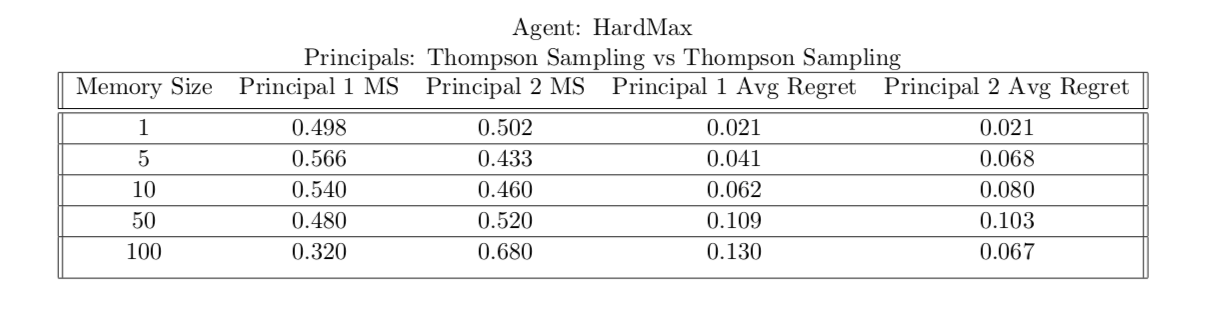
\includegraphics[scale=0.5]{memory_exp}
\end{itemize}
\end{frame}
%
\begin{frame}
{Experiment 3 - Tuning SoftMax}
\begin{itemize}
\item SoftMax is great!
\end{itemize}
\end{frame}
%
\begin{frame}
{Experiment 4 - Prior or Algorithm}
\begin{itemize}
\item The purpose of this experiment was to attempt to figure out if it's better to use a better learning algorithm matters more or have better initial information.
\item Ran simulations competing StaticGreedy (with almost correct beliefs) vs Thompson Sampling (with perverse beliefs) with $K = 10$
\item StaticGreedy had highest expected mean on the 2nd best arm, but Thompson Sampling had priors that thought the worst arms were the best and that the best arms were very bad. Who wins?
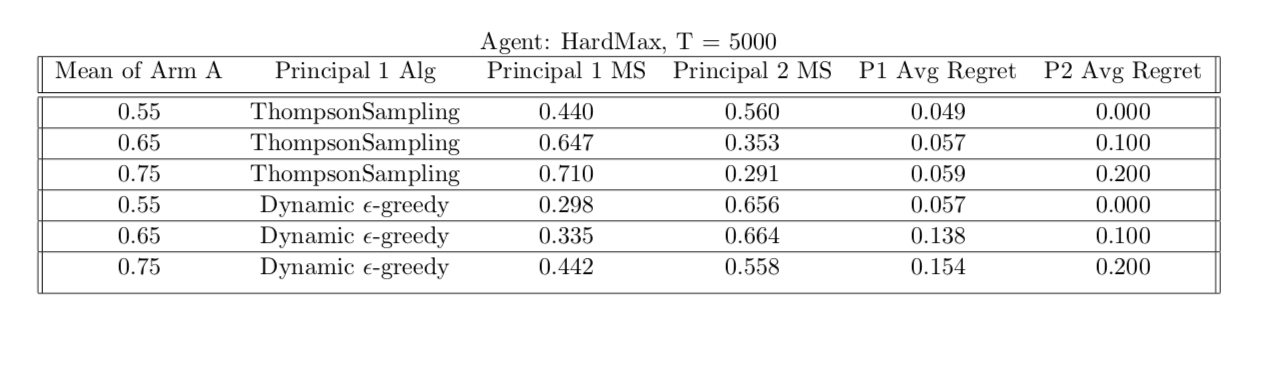
\includegraphics[scale=0.5]{prior_vs_alg_1}
\end{itemize}
\end{frame}
%
\begin{frame}
{Experiment 4 -  Prior or Algorithm Cont'd}
\begin{itemize}
\item What if we drastically reduce the number of periods in the simulation? \\
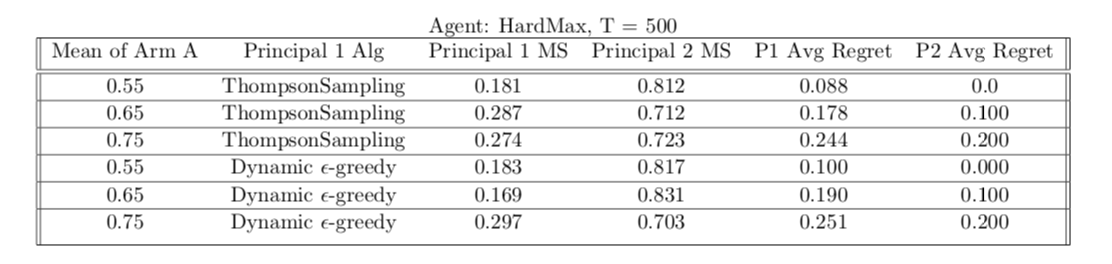
\includegraphics[scale=0.5]{prior_vs_alg_2}
\item Given enough time, the algorithms that explore will catch up, but if we have sufficiently few periods then better initial information seems to win (according to our parameterization)
\end{itemize}
\end{frame}
%
\begin{frame}
{Additional Considerations}
\begin{itemize}
\item What if we gave the principals free information at the start by giving them $N$ agents? Some simulations showed that there was no difference.
\item What if we made the rewards of the agents separate from the rewards of the principals?
\end{itemize}
\end{frame}
\end{document}
